\section{Representaciones gráficas.}

\subsection{Bidimensional.}

Podemos representar cualquier cubriz como una serie de matrices separadas por barras verticales, donde cada matriz sería una ``rodaja'' ($k=1$, $k=2$...) de la cubriz. Esta es la representación estándar para imprenta.

\[ \left(
\begin{array}{c c c | c | c c c}
	\alpha_{111} & \cdots & \alpha_{1n1} &        & \alpha_{11o} & \cdots & \alpha_{1no} \\
	\vdots       &        & \vdots       & \cdots & \vdots       &        & \vdots       \\
	\alpha_{m11} & \cdots & \alpha_{mn1} &        & \alpha_{m1o} & \cdots & \alpha_{mno} \\
\end{array} \right)
\]

\subsection{Tridimensional superficial.}

En ocasiones bastará con una vista panorámica de la cubriz que no entre en detalle. Para este fin podemos organizar cada elemento en vóxeles que constituyan un prisma rectangular.

\begin{figure}[H]
	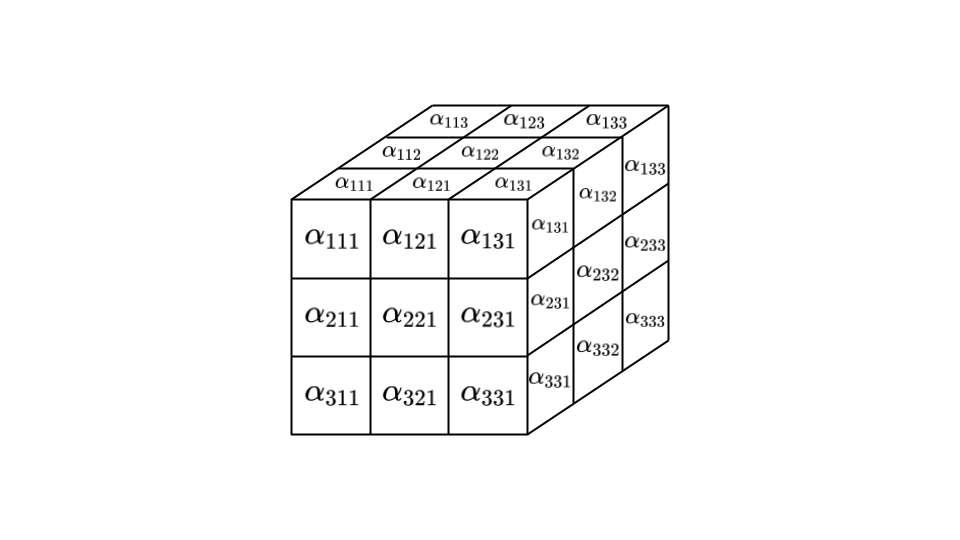
\includegraphics[width=\linewidth]{media/tridimensional_sup.png}
	\caption{Representación tridimensional superficial de una cubriz con elementos $\alpha_{ijk}$.}
\end{figure}

\newpage

\subsection{Tridimensional completa.}

Para una vista completa pero que conserve la estructura tridimensional, podemos separar cada ``rodaja'' de la cubriz a lo largo de un subíndice. Esta representación puede asistir en el reconocimiento de patrones.

\begin{figure}[H]
	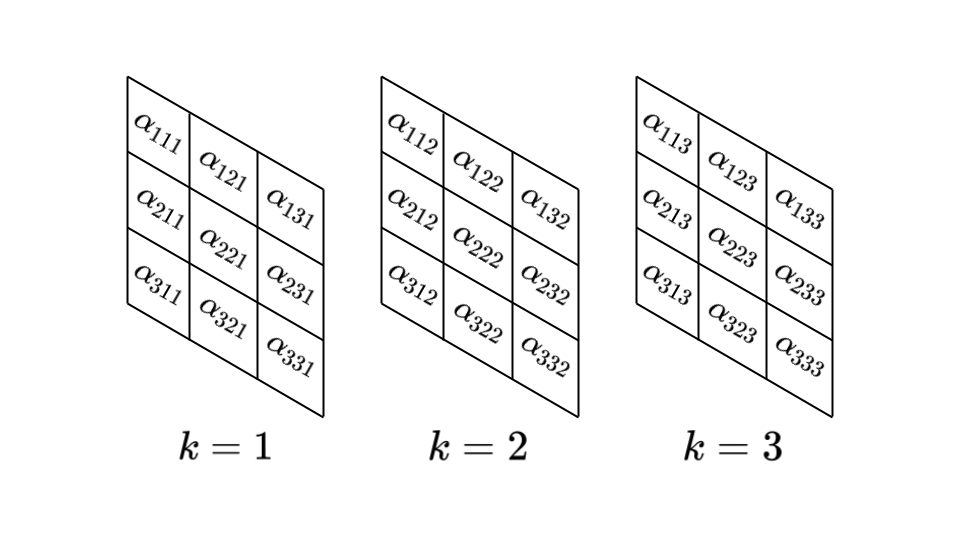
\includegraphics[width=\linewidth]{media/tridimensional_comp.png}
	\caption{Representación tridimensional completa de una cubriz con elementos $\alpha_{ijk}$.}
\end{figure}

\subsection{Producto.}

Bajo la definición ofrecida, el elemento $ijk$ de la cubriz $\Delta = (AB\Gamma)$ será igual al producto de la fila $i$ de $A$ por la columna $j$ de $B$ por la ``profundidad'' $k$ de $\Gamma$.

\begin{figure}[H]
	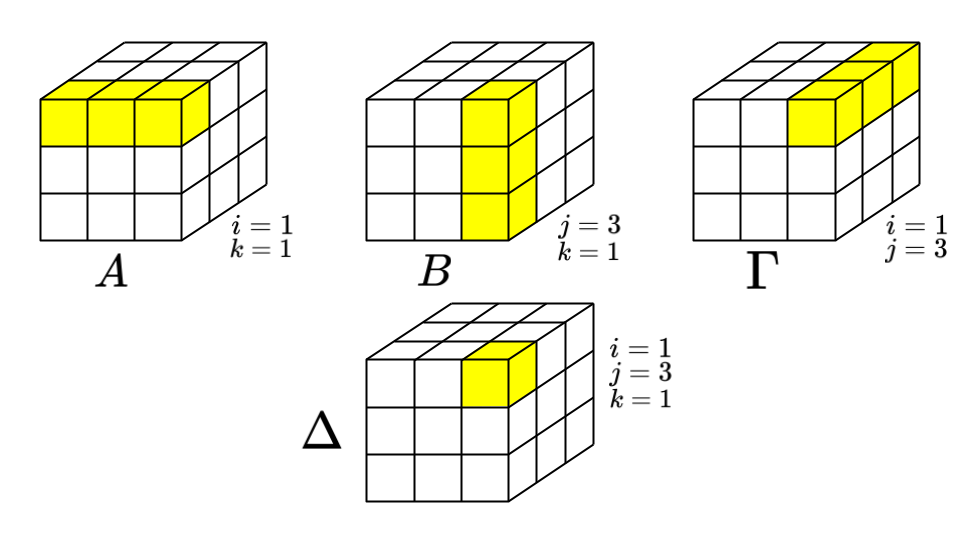
\includegraphics[width=\linewidth]{media/product.png}
	\caption{Representación tridimensional superficial del producto $\Delta = (AB\Gamma)$.}
\end{figure}

Esto explica las restricciones que marcan las dimensiones. En el proceso iterativo de la suma, es necesario que coincidan el número de columnas de $A$ ($n$), el número de filas de $B$ ($p$) y el número de ``profundidades'' de $\Gamma$ ($u$). Además, $\Delta$ no podrá tener más filas que $A$ ni que $\Gamma$ (de lo contrario, accederíamos a valores inexistentes), ni más columnas que $B$ o $\Gamma$, ni más ``profundidades'' que $A$ o $B$.
